\documentclass[aip,cha,reprint,amsmath,amssymb]{revtex4-2}

\usepackage{graphicx}
\usepackage{bm}
\usepackage{amsthm}
\usepackage[colorlinks=true,allcolors=blue]{hyperref}

\newtheorem{proposition}{Proposition}
\newtheorem{theorem}[proposition]{Theorem}
\newtheorem{corollary}[proposition]{Corollary}
\newtheorem{lemma}[proposition]{Lemma}
\theoremstyle{remark}
\newtheorem{remark}{Remark}

\newcommand{\one}{\mathbf 1}
\newcommand{\corr}{\operatorname{corr}}
\newcommand{\GSR}{\operatorname{GSR}}
\newcommand{\diag}{\operatorname{diag}}
\newcommand{\FC}{\mathrm{FC}}

\begin{document}

\title{The global-mode confound: what fitted whole-brain models can and cannot tell about the distance to a bifurcation}

\author{Yuriria Cort\'es Poza}
\thanks{ORCID: \href{https://orcid.org/0000-0003-1856-9206}{0000-0003-1856-9206}}
\affiliation{Instituto de Investigaciones en Matem\'aticas Aplicadas y en Sistemas (IIMAS), Universidad Nacional Aut\'onoma de M\'exico, Mexico City, Mexico}

\date{\today}

\begin{abstract}
Whole-brain models of coupled Stuart--Landau oscillators are fitted to resting-state functional connectivity (FC), and the fitted operating point is read as the brain's distance to a Hopf bifurcation. We separate two versions of this distance. The physical rate $\delta$ is not identifiable from zero-lag FC, which is invariant under a rescaling of time and under a common oscillation frequency. The dimensionless distance $\theta$, the ratio of damping to coupling, is identifiable in principle given the connectome, but confounded in practice. With excitatory coupling the mode that loses stability first is a positive Perron vector, bounded away from orthogonality to the uniform vector; with diffusive coupling it is the uniform vector. Near the bifurcation $\theta$ therefore enters FC only through its global level, where a uniform global component of any origin mimics it, and global signal regression removes 99.5\% of its first-order effect on a human connectome. We call this the \emph{global-mode confound}. In 800 Human Connectome Project sessions, the FC-based index $\kappa$, the slowest relaxation rate relative to the mean rate, is almost a function of mean FC without regression ($r=-0.995$ for $\log\kappa$) and becomes model-dependent with it. Simulations of the full nonlinear model confirm the confound up to the bifurcation. In data simulated from the model, the autocorrelation of the global signal recovers $\delta$ where FC cannot.
\end{abstract}

\maketitle

\begin{quotation}
\noindent\textbf{%
A popular way to ask whether the resting brain sits close to an instability is to fit a network of noisy oscillators to the pattern of correlations between brain regions, and then read off how close the fitted network is to its bifurcation. We show that this data cannot give the distance in physical units, and gives a relative distance only in principle. The correlation pattern has no clock, so it cannot tell a slow system from a fast one; at best it fixes the distance relative to the strength of the coupling. Moreover, in networks with excitatory coupling, the pattern that becomes slow at the bifurcation is essentially the average of all regions, the ``global signal''. A change in the relative distance therefore looks like a change in the amplitude of a global signal with equal weights on all regions. Global signals in brain imaging also arise from breathing, arousal and head motion, and are routinely regressed out; within the model, regressing them out removes the information as well. We prove these statements for the linearized model, confirm them on a large human data set, and indicate what measurements could answer the question.}
\end{quotation}

%======================================================================
\section{Introduction}\label{sec:intro}

The hypothesis that the brain operates near a critical point has motivated two decades of work, from neuronal avalanches to large-scale imaging~\cite{OByrne2022,Wilting2018}. At the scale of whole-brain imaging the hypothesis is usually tested with models: a network of nonlinear oscillators, one per brain region, is coupled through the anatomical connectome and fitted to resting-state functional magnetic resonance imaging (fMRI)~\cite{Cabral2011}. The most widely used local dynamics is the normal form of a supercritical Hopf bifurcation, the Stuart--Landau oscillator, whose bifurcation parameter $a_j$ and a global coupling $G$ are adjusted until simulated and empirical functional connectivity (FC), the matrix of zero-lag correlations between regional signals, agree~\cite{Deco2017dynamics,Deco2017single,PonceAlvarez2024}. The fitted operating point is then interpreted: best fits near $a_j\approx0$ are read as evidence that the brain lies at the edge of the bifurcation~\cite{Deco2017dynamics}, and shifts of $a_j$ between brain states as movements towards or away from it; for example, slow-wave sleep has been described as a shift of the working point from the edge of the transition to a stable focus~\cite{Jobst2017}. Related arguments with other local dynamics reach the same conclusion: resting-state networks emerge in a model of the connectome only when it is tuned to criticality~\cite{Haimovici2013}.

There is a tension in this programme. Criticality is a statement about time: at a bifurcation a mode loses its damping and its relaxation time diverges. Zero-lag FC is a normalized covariance and contains no unit of time. It is not obvious that a quantity without a clock can measure a rate.

This paper shows that it cannot measure the rate, and that the dimensionless distance it can identify in principle is confounded in practice. We keep the two apart throughout: $\delta$ denotes the physical distance to the bifurcation, in $\mathrm s^{-1}$, and $\theta$ (or the index $\kappa$ of Sec.~\ref{sec:model}) a dimensionless distance measured in units of the coupling. In linearized whole-brain models with excitatory coupling, zero-lag FC is blind to the time scale, so $\delta$ is out of reach. The mode that becomes critical is, up to an explicit Perron--Frobenius bound, the global signal. Near the bifurcation, $\theta$ therefore enters FC only through the global level of correlation. There it is indistinguishable from the amplitude of any global component with uniform loading that is unrelated to the dynamics, and global signal regression (GSR), the standard remedy for such components~\cite{Murphy2017,Liu2017}, removes it together with the component. We call this coincidence of the critical mode with the global signal the \emph{global-mode confound}.

The simplest example already shows both effects. Take a ring of identical damped oscillators with diffusive coupling (Fig.~\ref{fig:ring}). Speeding up every rate by a factor of four shortens the autocorrelation of every node by the same factor, yet the FC matrix does not change at all. The slowest mode, which decides how close the ring is to instability, is the uniform vector: every node moves together. Its rate $\theta$ is the distance to the bifurcation in units of the coupling, and near the bifurcation it affects FC, to first order, only through how strongly all nodes are correlated with all others.

\begin{figure*}
  \centering
  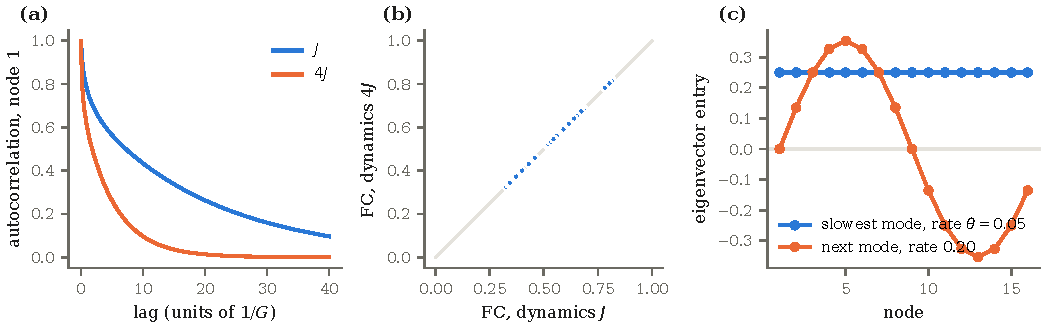
\includegraphics[width=\textwidth]{figures/fig1_ring.pdf}
  \caption{The two obstructions on a ring of $N=16$ diffusively coupled nodes with one chord, homogeneous ratio $\theta=0.05$. (a) Autocorrelation of node 1 for the linearized dynamics $J=-(\theta I+L)$ and for $4J$: the time scale changes by a factor of four. (b) The FC matrices of the two systems coincide entry by entry (Proposition~\ref{prop:rescale}). (c) Eigenvectors of $\theta I+L$: the slowest mode, whose rate $\theta$ is the distance to the bifurcation, is the uniform vector (Proposition~\ref{prop:diffusive}); the next mode decays four times faster.}
  \label{fig:ring}
\end{figure*}

Our results are of two kinds. The first is a precise account of what zero-lag FC can identify. Proposition~\ref{prop:rescale} shows that FC is invariant under the rescaling $(a,\omega,G)\mapsto c(a,\omega,G)$, in the full nonlinear model and not only in its linearization, so the distance to the bifurcation in units of $\mathrm{s}^{-1}$ is not identifiable. Proposition~\ref{prop:omega} shows that a common oscillation frequency drops out exactly. Corollary~\ref{cor:closed} gives closed forms for the linearized FC and identifies it with a Gaussian graphical model; only partial correlations, and, when the coupling matrix is known, the ratios $\theta_j=|a_j|/G$, are identifiable. Parts of this are known in other guises: closed forms relating structural to functional connectivity~\cite{Galan2008,Saggio2016,Abdelnour2014}, the linearization of the Hopf model~\cite{PonceAlvarez2024}, the need for time-lagged covariances, or additional sparsity assumptions, to estimate effective connectivity~\cite{Gilson2016,Schiefer2018}, and, above the bifurcation, an empirical invariance of the fit to phase-based connectivity along curves $K\sim\sqrt\lambda$ of coupling against excitability~\cite{Alexandersen2025}. We state them in the form needed for the second kind of result.

The second kind is the global-mode confound itself, and its central statement is Theorem~\ref{thm:confound}. Whenever the zero-lag covariance near the bifurcation is dominated by a positive critical vector $v$, FC tends to $\one\one^\top$ along a fixed direction, and regression on \emph{any} positively weighted global signal cancels the divergent part of the critical mode exactly, leaving a limit that does not depend on the distance to the bifurcation. The hypothesis holds for diffusive and additive coupling (Propositions~\ref{prop:perron} and~\ref{prop:diffusive}) and, by Corollary~\ref{cor:nonnormal}, for directed, non-normal coupling, where the divergent variance lies along the right critical vector. Proposition~\ref{prop:left} adds the dynamical counterpart: the projection on the \emph{left} critical vector is an exact Ornstein--Uhlenbeck process with rate $\delta$. For diffusive coupling, Proposition~\ref{prop:gsr} makes the theorem quantitative: $\FC=\one\one^\top-\tfrac{N\theta}{2}\Omega+O(\theta^2)$, with $\Omega$ the effective-resistance matrix of the graph, a global artefact of variance $\sigma^2$ is equivalent to replacing $\theta$ by $\theta/(1+N\sigma^2\theta)$, and GSR removes 99.5\% of the first-order sensitivity on a human connectome.

These statements explain three observations in the literature that have so far been reported separately. Aquino and co-authors found that the accuracy of several whole-brain models tracks how well they fit the global signal, and that a two-parameter model does as well~\cite{Aquino2022}. Fitted operating points disagree between studies, just below the bifurcation in some~\cite{Deco2017dynamics} and arbitrarily far beyond it in others~\cite{Alexandersen2025}, and both report degeneracies of the fit: beyond a critical coupling the optimal regional bifurcation parameters ``remain the same, only scaled''~\cite{Deco2017dynamics}, and above the bifurcation the fit depends only on $K/\sqrt\lambda$~\cite{Alexandersen2025}. Below the bifurcation, Corollary~\ref{cor:closed} shows that a whole curve of operating points produces the same FC. And the FC dynamics used to select $G$ are largely reproduced by stationary linear processes~\cite{Liegeois2017}. We test each prediction on two data sets from the Human Connectome Project, time series from 7 subjects and FC from 200 subjects in 4 sessions each. We also check the theory in the full nonlinear model, where the confound holds up to the bifurcation and, above it, persists for a common frequency but weakens when frequencies are heterogeneous, and show, in data simulated from the model, that the autocorrelation of the global signal recovers $\delta$ along a family of systems with identical FC.

Section~\ref{sec:model} introduces the model and proves the identifiability results. Section~\ref{sec:confound} proves the global-mode confound. Section~\ref{sec:empirical} tests the predictions on data, and Sec.~\ref{sec:discussion} discusses what can be identified, what cannot, and which measurements could close the gap.

%======================================================================
\section{Model and identifiability}\label{sec:model}

\subsection{The whole-brain Stuart--Landau model}

Each of $N$ regions carries a complex amplitude $z_j$ that obeys
\begin{multline}\label{eq:sl}
  \mathrm dz_j=\Bigl[(a_j+i\omega_j)z_j-|z_j|^2z_j+G\sum_{k}M_{jk}z_k\Bigr]\mathrm dt\\
  +\beta\,(\mathrm dW^x_j+i\,\mathrm dW^y_j),
\end{multline}
where $a_j$ is the local bifurcation parameter, $\omega_j$ the intrinsic angular frequency, $G\ge0$ the global coupling, $\beta$ the noise amplitude and $W^x_j,W^y_j$ independent standard Wiener processes. The observed regional signal is $x_j=\operatorname{Re}z_j$. The coupling matrix is either \emph{diffusive}, $M=-L$ with $L=\diag(C\one)-C$ the Laplacian of the non-negative connectome $C$, as in Refs.~\onlinecite{Deco2017dynamics,PonceAlvarez2024}, or \emph{additive}, $M=C$. We say the coupling is \emph{excitatory} when $M$ is Metzler (non-negative off the diagonal); both choices are.

Below the bifurcation the origin is stable and, for small noise, Eq.~\eqref{eq:sl} is well approximated by its linearization~\cite{PonceAlvarez2024}. Writing $A=\diag(a)+GM$ and $\Omega_\omega=\diag(\omega)$, the linearized system is the complex Ornstein--Uhlenbeck process $\mathrm dz=(A+i\Omega_\omega)z\,\mathrm dt+\beta\,\mathrm d\mathbf W$, or, in real coordinates,
\begin{equation}\label{eq:jac}
  \mathrm d\begin{pmatrix}x\\y\end{pmatrix}=J\begin{pmatrix}x\\y\end{pmatrix}\mathrm dt+\beta\,\mathrm d\mathbf W,\qquad
  J=\begin{pmatrix}A&-\Omega_\omega\\ \Omega_\omega&A\end{pmatrix}.
\end{equation}
Its stationary covariance $\Sigma$ solves the Lyapunov equation $J\Sigma+\Sigma J^\top+\beta^2I=0$, and $\FC=\corr(\Sigma_{xx})$, where $\corr(S)=D_S^{-1/2}SD_S^{-1/2}$ and $D_S=\diag(S)$. The \emph{distance to the bifurcation} is $\delta=-\max\operatorname{Re}\operatorname{spec}(J)$, in units of $\mathrm{s}^{-1}$. For the empirical data in Sec.~\ref{sec:empirical}, the linearized FC agreed with simulations of Eq.~\eqref{eq:sl} with $r>0.98$ over the range of operating points we fitted.

\subsection{Time rescaling}

\begin{proposition}[Time rescaling]\label{prop:rescale}
Let $z(t)$ be a stationary solution of Eq.~\eqref{eq:sl} with parameters $(a,\omega,G,\beta)$ and let $c>0$. Then $\sqrt c\,z(ct)$ is a stationary solution of Eq.~\eqref{eq:sl} with parameters $(ca,c\omega,cG,c\beta)$. Consequently, every statistic of the stationary distribution that is invariant under a common scaling of the signals, in particular zero-lag FC, takes the same value at $(a,\omega,G)$ and at $(ca,c\omega,cG)$, while $\delta$ is multiplied by $c$.
\end{proposition}

\begin{proof}
Set $u(t)=\sqrt c\,z(ct)$. Then $\mathrm du=\sqrt c\,c\bigl[(a+i\omega)z-|z|^2z+GMz\bigr](ct)\,\mathrm dt+\sqrt c\,\beta\,\mathrm d\mathbf W(ct)$. Since $\sqrt c\,z=u$ and $c|z|^2=|u|^2$, the drift equals $\bigl[(ca+ic\omega)u-|u|^2u+cGMu\bigr]\mathrm dt$. The process $\mathbf W(ct)$ has the law of $\sqrt c\,\widetilde{\mathbf W}(t)$ for a standard Wiener process $\widetilde{\mathbf W}$, so the noise term is $c\beta\,\mathrm d\widetilde{\mathbf W}$. The marginal law of $u(t)$ is that of $\sqrt c\,z(0)$, and correlations are invariant under the factor $\sqrt c$. Finally $\operatorname{spec}J$ scales by $c$ because $J$ is linear in $(a,\omega,G)$.
\end{proof}

In the linearization $\beta$ only fixes the overall amplitude, which FC discards. In the full model it does not: $\beta$ sets the noise level relative to the amplitude at which the cubic term saturates, and with $\beta$ held fixed FC does change along $(ca,c\omega,cG)$. In a check on the AAL2 group connectome ($G=0.2$, empirical frequencies, $c=4$), the change was 2.3 times the sampling noise at $a=-0.01$ and 32 times at $a=0.005$ (\texttt{src/beta\_check.py}), whereas with $\beta$ rescaled as in the proposition it was within the noise. Since BOLD signals carry no absolute amplitude scale, $\beta$ is itself a free parameter. An FC-based fit can therefore at best determine $(a,\omega,G,\beta)$ up to the common factor of Proposition~\ref{prop:rescale}; fixing $\beta$ by convention, as is usual, fixes the scale of the fitted $\delta$ by the same convention rather than by the data. The statement is exact for the unfiltered signal. A band-pass filter with fixed cut-offs in hertz breaks the invariance, so filtered FC does carry information about the time scale, but only through the shape of the filter. In Sec.~\ref{sec:fit} we show that in practice this information is too weak to pin down $\delta$.

\subsection{A common frequency drops out}

\begin{proposition}[Common frequency]\label{prop:omega}
If $\omega_j=\omega$ for all $j$, the stationary law of $z(t)$ at a fixed time, and hence zero-lag FC, does not depend on $\omega$. This holds for Eq.~\eqref{eq:sl} and for its linearization.
\end{proposition}

\begin{proof}
Let $u(t)=e^{-i\omega t}z(t)$. Because the cubic term and the coupling commute with a global phase rotation,
$\mathrm du=\bigl[a\odot u-|u|^2\odot u+GMu\bigr]\mathrm dt+\beta e^{-i\omega t}\mathrm d\mathbf W$, where $\odot$ is the entrywise product. Circular complex white noise is invariant in law under a deterministic rotation, so $u$ is a solution of Eq.~\eqref{eq:sl} with $\omega=0$. That system is equivariant under $u\mapsto e^{i\phi}u$, and so is its noise, so its stationary law is rotation invariant; the stationary law is unique because the noise acts on every coordinate and the cubic term confines the dynamics (for the linearization, because $A$ is Hurwitz). Hence $z(t)=e^{i\omega t}u(t)$ has the same marginal law as $u(t)$.
\end{proof}

Heterogeneous frequencies do enter FC, but weakly in the diffusive model: in our fits, setting $\omega_j=0$ (a multivariate Ornstein--Uhlenbeck model without oscillation) reproduced FC as well as the Hopf model did (Sec.~\ref{sec:fit}).

\subsection{Closed forms and the graphical-model reading}

From now on, $C$ is symmetric and the frequency is common. By Proposition~\ref{prop:omega} we may set $\omega=0$. Then $x$ and $y$ are independent, $A$ is symmetric negative definite, and the Lyapunov equation gives $\Sigma_{xx}=-\tfrac{\beta^2}{2}A^{-1}$.

\begin{corollary}[Closed forms and identifiability]\label{cor:closed}
Let $C$ be symmetric, non-negative and irreducible, and let the frequency be common.
\begin{enumerate}
  \item[(i)] Diffusive coupling: $\FC=\corr\bigl[(\diag\theta+L)^{-1}\bigr]$ with $\theta_j=|a_j|/G$. Additive coupling with homogeneous $a$: $\FC=\corr\bigl[(I-\rho\hat C)^{-1}\bigr]$ with $\hat C=C/\lambda_{\max}(C)$ and $\rho=G\lambda_{\max}(C)/|a|<1$; the bifurcation is at $\rho=1$.
  \item[(ii)] In both cases $x$ is a Gaussian vector with precision matrix proportional to $K=\diag(q)-C$, with $q_j=\theta_j+\sum_kC_{jk}$ (diffusive) or $q_j=|a_j|/G$ (additive). For any precision $K$ and any positive diagonal $D$, $\corr(K^{-1})=\corr\bigl((DKD)^{-1}\bigr)$, and FC determines $K$ exactly up to $K\mapsto DKD$. Hence FC identifies precisely the partial correlations $\pi_{ij}=-K_{ij}/\sqrt{K_{ii}K_{jj}}$.
  \item[(iii)] If $C$ is known and its graph is connected and not bipartite, then $q$, and hence every $\theta_j$, is identifiable from FC. If $C$ is a free parameter, no function of $q$ that is not invariant under $q\mapsto D^2q$ is identifiable; for additive coupling this holds for every positive diagonal $D$, and for diffusive coupling, where the transformed model must keep $\theta\ge0$, for $D$ close to the identity when $\theta>0$. In neither case is $\delta$ in $\mathrm{s}^{-1}$ identifiable.
\end{enumerate}
\end{corollary}

\begin{proof}
(i) For diffusive coupling, $A=-\diag|a|-GL=-G(\diag\theta+L)$; for additive coupling, $A=-|a|(I-\rho\hat C)$. Positive factors disappear in $\corr$.
(ii) $\Sigma_{xx}\propto K^{-1}$ with $K$ as stated, because $L=\diag(C\one)-C$. The identity $(DKD)^{-1}=D^{-1}K^{-1}D^{-1}$ gives the invariance. Conversely, if $\corr(K^{-1})=\corr(K'^{-1})=F$, then $K^{-1}=E F E$ and $K'^{-1}=E'FE'$ for positive diagonal $E,E'$, so $K'=(E^{-1}E')^{-1}K(E^{-1}E')^{-1}$. Partial correlations are invariant under $K\mapsto DKD$, and they determine $K$ up to that transformation.
(iii) For an edge $(i,j)$, $\pi_{ij}^2=C_{ij}^2/(q_iq_j)$, so the products $q_iq_j$ are known on every edge. On a connected graph these products fix $q$ up to $q_i\mapsto tq_i$ on one class of a bipartition and $q_i\mapsto q_i/t$ on the other; an odd cycle forces $t=1$. If $C$ is free, $DKD=\diag(D^2q)-DCD$ with $DCD$ again symmetric and non-negative, so $(q,C)$ and $(D^2q,DCD)$ give the same FC; for diffusive coupling the implied $\theta'=D^2q-DCD\one$ is non-negative for $D$ near $I$ when $\theta>0$. The last claim is Proposition~\ref{prop:rescale}.
\end{proof}

Part (iii) separates two regimes that are often conflated. With a fixed structural connectome, the dimensionless ratios $\theta_j$ are identifiable in principle; with a fitted effective connectivity they are not, because the fit can absorb any diagonal rescaling. Even in the first regime, only the ratio of damping to coupling is fixed. An analogous degeneracy above the bifurcation, where the fit to phase-lag connectivity depends only on the ratio $K/\sqrt\lambda$ of coupling to excitability, was found empirically in Ref.~\onlinecite{Alexandersen2025}; that regime lies outside our linear analysis. In neither regime can a fitted distance from $a=0$ be read as a rate.

For homogeneous diffusive damping, $\delta=G\theta$, and the scale-free version of the distance to the bifurcation is $\theta$ itself. More generally we use the index $\kappa=\mu_{\min}/\bar\mu$, the ratio of the slowest decay rate to the mean decay rate of $-A$. It is invariant under Proposition~\ref{prop:rescale} and vanishes at the bifurcation. For additive coupling with homogeneous $a$, $\operatorname{tr}C=0$ gives $\kappa=1-\rho$.

%======================================================================
\section{The global-mode confound}\label{sec:confound}

\subsection{The critical mode is positive}

\begin{proposition}[Critical mode under excitatory coupling]\label{prop:perron}
Let $A=\diag(a)+GM$ with $M$ Metzler and irreducible, and let the frequency be common, so that the real parts of the eigenvalues of $J$ are those of $A$. Then the eigenvalue of $A$ with largest real part, $-\delta$, is real and simple, and its eigenvector $v$ can be chosen with all entries positive. With $v_{\min}=\min_jv_j$ and $v_{\max}=\max_jv_j$,
\begin{equation}\label{eq:polya}
  \cos\angle(v,\one)=\frac{\one^\top v}{\sqrt N\,\|v\|}\ \ge\ \frac{2\sqrt{v_{\min}v_{\max}}}{v_{\min}+v_{\max}}.
\end{equation}
If moreover $A$ is symmetric, $\Sigma_{xx}=\tfrac{\beta^2}{2}\sum_k\mu_k^{-1}u_ku_k^\top$ in the orthonormal eigenbasis $\{u_k\}$ of $-A$, with $u_1=v/\|v\|$ and $\mu_1=\delta$, so the fraction of the total variance carried by $v$ tends to one as $\delta\to0$ with the remaining rates bounded away from zero.
\end{proposition}

\begin{proof}
For $s$ large, $A+sI$ is non-negative and irreducible, and the Perron--Frobenius theorem~\cite{Berman1994} gives a simple real eigenvalue of maximal modulus, which for $A$ is the eigenvalue of maximal real part, with a positive eigenvector. For \eqref{eq:polya}, which is the Pólya--Szegő inequality~\cite{PolyaSzego1925}, note that $(v_j-v_{\min})(v_{\max}-v_j)\ge0$ gives $v_j^2+v_{\min}v_{\max}\le(v_{\min}+v_{\max})v_j$. Summing over $j$ and using $2\sqrt{N v_{\min}v_{\max}}\,\|v\|\le\|v\|^2+Nv_{\min}v_{\max}$ yields $2\sqrt{Nv_{\min}v_{\max}}\,\|v\|\le(v_{\min}+v_{\max})\one^\top v$. The variance statement follows from $\Sigma_{xx}=-\tfrac{\beta^2}2A^{-1}$.
\end{proof}

The bound \eqref{eq:polya} depends only on the spread of the Perron vector. For additive coupling with homogeneous $a$, $v$ is the Perron vector of $C$; for the group structural connectome of Sec.~\ref{sec:empirical}, $\cos\angle(v,\one)=0.82$, and $0.989$ after the compressive transformation of the weights selected by the fit (Sec.~\ref{sec:additive}).

\subsection{Diffusive coupling: the critical mode is the global signal}

\begin{proposition}[Diffusive coupling]\label{prop:diffusive}
Let $M=-L$ with $C$ symmetric, the graph connected and the frequency common, and let $0=\lambda_1<\lambda_2\le\dots\le\lambda_N$ be the eigenvalues of $L$. Then $\delta/G$ is the smallest eigenvalue of $\diag\theta+L$, and $\theta_{\min}\le\delta/G\le\bar\theta$, where $\bar\theta$ is the mean of $\theta$. If $\theta$ is homogeneous, the critical mode is exactly $\one/\sqrt N$ and $\delta=G\theta$. In general, its angle $\phi$ to $\one$ satisfies
\begin{equation}\label{eq:dk}
  \sin\phi\le\frac{\theta_{\max}-\theta_{\min}}{\lambda_2}.
\end{equation}
\end{proposition}

\begin{proof}
$-A=G(\diag\theta+L)$. The lower bound holds because $L\succeq0$; the upper bound is the Rayleigh quotient at $\one$. For homogeneous $\theta$, $(\theta I+L)\one=\theta\one$ and $\theta$ is the smallest eigenvalue because $L\succeq0$. In general write $\diag\theta+L=(\tilde\theta I+L)+E$ with $\tilde\theta=(\theta_{\max}+\theta_{\min})/2$ and $E=\diag(\theta-\tilde\theta)$, so $\|E\|_{\mathrm{op}}=(\theta_{\max}-\theta_{\min})/2$. The unperturbed matrix has its smallest eigenvalue $\tilde\theta$, eigenvector $\one$, separated from the rest of the spectrum by $\lambda_2$. The Davis--Kahan bound in the form of Theorem~2 of Ref.~\onlinecite{Yu2015}, which requires only symmetry and a gap in the unperturbed spectrum, gives $\sin\phi\le2\|E\|_{\mathrm{op}}/\lambda_2$.
\end{proof}

The slowest mode of the diffusive model is therefore, up to the heterogeneity of the damping relative to the spectral gap, the average of all regions. It is the mode whose variance diverges at the bifurcation (Proposition~\ref{prop:perron}), and it is also, by construction, the mode removed by global signal regression. The next subsection quantifies the consequences.

% General global-mode theorem (any symmetric excitatory coupling, homogeneous damping).
% Numerical check: src/theorem_general_check.py

\subsection{The confound for general excitatory coupling}\label{sec:general}

The next result states the confound without assuming that the critical mode is uniform. Its
hypothesis covers both couplings of Corollary~\ref{cor:closed} with homogeneous damping. For
diffusive coupling, $S\propto(\theta I+L)^{-1}$ has critical rate $\varepsilon=\theta$ and
$v=\one/\sqrt N$. For additive coupling, $S\propto(I-\rho\hat C)^{-1}$ has critical rate
$\varepsilon=1-\rho=\kappa$ and $v$ is the Perron vector of $C$. In both cases the eigenvectors do not
depend on the distance to the bifurcation, and
\begin{equation}\label{eq:S-eps}
  S(\varepsilon)=\varepsilon^{-1}vv^\top+R(\varepsilon),\qquad R(\varepsilon)v=0,
\end{equation}
with $v>0$, $\|v\|=1$, and $R$ real-analytic at $\varepsilon=0$ with $R(0)\succeq0$ and $\ker R(0)=\operatorname{span}\{v\}$.
A \emph{global signal} is any weighted average $g=w^\top x$ with $w$ depending analytically on
$\varepsilon$ and $w(0)^\top v\ne0$; positive weights always qualify, because $v>0$. Regressing $g$
out of the standardized signals is the GSR of Eq.~\eqref{eq:gsr}. It corresponds to
$w=D_S^{-1/2}\one\propto D_v^{-1}\one+O(\varepsilon)$, while regressing out the mean of the raw
signals corresponds to $w=\one$.

\begin{theorem}[Global-mode confound]\label{thm:confound}
Assume \eqref{eq:S-eps} and let $F(\varepsilon)=\corr S(\varepsilon)$. Write
$\tilde R=D_v^{-1}R(0)D_v^{-1}$ and $\Omega_v(i,j)=\tilde R_{ii}+\tilde R_{jj}-2\tilde R_{ij}$. As $\varepsilon\downarrow0$:
\begin{enumerate}
  \item[(a)] $F(\varepsilon)=\one\one^\top-\tfrac{\varepsilon}{2}\,\Omega_v+O(\varepsilon^2)$;
  \item[(b)] for every global signal $w$, the covariance of the residuals of $x$ after regression on $w^\top x$ satisfies
  \[
    Q(\varepsilon)=\Pi R(0)\Pi^\top+O(\varepsilon),\qquad \Pi=I-\frac{v\,w(0)^\top}{w(0)^\top v},
  \]
  so the FC after regression converges to $\corr\bigl(\Pi R(0)\Pi^\top\bigr)$, which does not depend on $\varepsilon$;
  \item[(c)] adding an independent component with loading $v$, $S\mapsto S+\sigma^2vv^\top$, is the same as replacing $\varepsilon$ by $\varepsilon_{\rm eff}$ in the singular part, $\varepsilon_{\rm eff}^{-1}=\varepsilon^{-1}+\sigma^2$, and changes $F$ by $O(\varepsilon\,\varepsilon_{\rm eff})$ relative to $F(\varepsilon_{\rm eff})$.
\end{enumerate}
The constants in (a) and (b) are controlled by $\max_i\tilde R_{ii}=\max_iR(0)_{ii}/v_i^2$, so the
expansions hold for $\varepsilon\ll\varepsilon^*:=1/\max_i\tilde R_{ii}$.
\end{theorem}

\begin{proof}
(a) Since $S_{ij}=\varepsilon^{-1}v_iv_j\bigl(1+\varepsilon\tilde R_{ij}+O(\varepsilon^2)\bigr)$ and $v_iv_j>0$,
\begin{align*}
  F_{ij}&=\frac{1+\varepsilon\tilde R_{ij}}{\sqrt{(1+\varepsilon\tilde R_{ii})(1+\varepsilon\tilde R_{jj})}}+O(\varepsilon^2)\\
  &=1-\tfrac{\varepsilon}{2}\Omega_v(i,j)+O(\varepsilon^2).
\end{align*}
(b) Write $c=v^\top w$, $r=R w$ and $\eta=\varepsilon\,w^\top r/c^2$. Then $Sw=\varepsilon^{-1}c\,v+r$ and $w^\top Sw=\varepsilon^{-1}c^2(1+\eta)$, because $v^\top r=0$. Expanding $Q=S-Sww^\top S/(w^\top Sw)$ gives the exact identity
\begin{multline*}
  Q=R-\frac{v r^\top+r v^\top}{c\,(1+\eta)}\\
  +\frac{w^\top r}{c^2(1+\eta)}\,vv^\top-\frac{\varepsilon\,rr^\top}{c^2(1+\eta)}.
\end{multline*}
The singular terms $\varepsilon^{-1}vv^\top$ cancel exactly. Letting $\varepsilon\to0$, so that $\eta\to0$, $w\to w(0)$ and $R\to R(0)$, yields $R(0)-\bigl(vr^\top+rv^\top\bigr)/c+(w^\top r/c^2)vv^\top=\Pi R(0)\Pi^\top$. The limit has positive diagonal unless some $\Pi^\top e_i$ lies in $\ker R(0)=\operatorname{span}\{v\}$, which fails for generic $w$, and $\corr$ is continuous there.
(c) $S+\sigma^2vv^\top=\varepsilon_{\rm eff}^{-1}vv^\top+R(\varepsilon)$, and $R(\varepsilon)-R(\varepsilon_{\rm eff})=O(\varepsilon)$ enters $F$ multiplied by $\varepsilon_{\rm eff}$, by (a).
\end{proof}

Three consequences deserve emphasis. First, part (b) does not require the critical mode to be close
to uniform. Any regression on a global signal with positive weights removes the divergent part of
the critical mode exactly, and after it FC no longer depends on the distance to the bifurcation at
leading order. The bound of Proposition~\ref{prop:perron} is not needed for this. Second, for
standardized signals the critical mode \emph{is} uniform at leading order: $D_S^{-1/2}v\propto\one+O(\varepsilon)$.
This is why mean FC tracks the distance to the bifurcation in both models (Sec.~\ref{sec:kappa}).
Third, Proposition~\ref{prop:perron} matters for (c). Physiological global components, whose
loading is roughly uniform, mimic a change of $\varepsilon$ to the extent that their loading overlaps
with $v$.

The window $\varepsilon^*$ can be narrow. For the Schaefer-100 group connectome,
$\varepsilon^*=2.9\times10^{-3}$ in units of $\theta$ for diffusive coupling. For additive coupling it
is $2.0\times10^{-4}$ in units of $\kappa$ for untransformed weights, whose Perron vector has
$v_{\min}/v_{\max}=0.05$, and $3.5\times10^{-3}$ after the compressive transformation
$\mathrm{SC}^{0.25}$. Outside the window the suppression by GSR is partial but already substantial.
For example, the sensitivity ratio of Proposition~\ref{prop:gsr} is 0.11 at $\theta=0.06$
(Fig.~\ref{fig:gsr}b).


% Proposition 5 (global signal regression near the bifurcation) and its proof.
% Numerical check: src/prop5_check.py
% Notation: L symmetric Laplacian of a connected weighted graph, eigenpairs
% 0 = lambda_1 < lambda_2 <= ... <= lambda_N, u_1 = N^{-1/2} 1; P = N^{-1} 1 1^T;
% L^+ Moore--Penrose pseudoinverse; corr(S) = D_S^{-1/2} S D_S^{-1/2}.

\subsection{The diffusive case quantified}\label{sec:diffusive-q}

For diffusive coupling the objects of Theorem~\ref{thm:confound} are explicit, and the first-order
correction after GSR can be computed. For homogeneous ratio $\theta=|a|/G$ and symmetric coupling, the
zero-lag covariance of the real parts is, up to a positive factor,
\begin{equation}\label{eq:S-theta}
  S(\theta)=(\theta I+L)^{-1}=\frac1\theta\,P+R(\theta),\qquad
  R(\theta)=\sum_{k\ge2}\frac{u_ku_k^{\top}}{\theta+\lambda_k},
\end{equation}
so that $R(\theta)\mathbf 1=0$ and $R(0)=L^{+}$. The critical mode is $\mathbf 1$ and its variance
$1/\theta$ diverges at the bifurcation. We write
$\Omega_{ij}=L^{+}_{ii}+L^{+}_{jj}-2L^{+}_{ij}$ for the effective resistance between nodes $i$ and $j$~\cite{Klein1993},
$\ell=\operatorname{diag}(L^{+})$ and $h=L^{+}\ell$.

\begin{proposition}[GSR near the bifurcation]\label{prop:gsr}
Let $L$ be the Laplacian of a connected weighted graph on $N$ nodes, let $F(\theta)=\operatorname{corr}S(\theta)$
with $S(\theta)$ as in \eqref{eq:S-theta}, and let $G(\theta)=\operatorname{GSR}(F(\theta))$. Then
$F$ and $G$ extend to real-analytic functions of $\theta$ on a neighbourhood of $\theta=0$, and as
$\theta\downarrow0$:
\begin{enumerate}
  \item[(a)] $F(\theta)=\mathbf 1\mathbf 1^{\top}-\dfrac{N\theta}{2}\,\Omega+O(\theta^{2})$;
  \item[(b)] $G(\theta)=\operatorname{corr}(L^{+})+\theta\,G_1+O(\theta^{2})$, where
  $G_1=\mathrm d\operatorname{corr}_{L^{+}}\bigl[-(L^{+})^{2}+\tfrac12(\mathbf 1h^{\top}+h\mathbf 1^{\top})\bigr]$;
  \item[(c)] consequently
  \[
    \lim_{\theta\downarrow0}
    \frac{\|\partial_{\log\theta}G\|}{\|\partial_{\log\theta}F\|}
    =\rho_\infty(L):=\frac{2\,\|G_1\|}{N\,\|\Omega\|},
  \]
  for any norm on the off-diagonal entries.
\end{enumerate}
Moreover, if a global component independent of $x$ is added, $S_\sigma=S+\sigma^{2}\mathbf 1\mathbf 1^{\top}$,
then
\begin{enumerate}
  \item[(d)] $\operatorname{corr}S_\sigma(\theta)=F(\theta_{\mathrm{eff}})+O(\theta\,\theta_{\mathrm{eff}})$ with
  $\theta_{\mathrm{eff}}^{-1}=\theta^{-1}+N\sigma^{2}$; and
  $\operatorname{GSR}(\operatorname{corr}S_\sigma(\theta))=\operatorname{corr}(L^{+})+O(\theta)$.
\end{enumerate}
\end{proposition}

In words, before GSR the only first-order trace of $\theta$ in $F$ is the global level
$\mathbf 1\mathbf 1^{\top}-F$. That level is proportional to a fixed matrix $\Omega$, and by (d) it
cannot be distinguished from the amplitude of an unrelated global component with uniform loading.
GSR removes that component together with the information. The limit $\operatorname{corr}(L^{+})$ does not depend on
$\theta$, and the residual sensitivity is reduced by the factor $\rho_\infty(L)$.

\begin{proof}
\emph{Analyticity.} Set $\varepsilon=N\theta$ and $T(\theta)=\theta S(\theta)=P+\theta R(\theta)$. Each
$\theta\mapsto(\theta+\lambda_k)^{-1}$ with $k\ge2$ is analytic on $|\theta|<\lambda_2$, so $T$ is
analytic there and $T(0)=P$ has diagonal $1/N>0$. The map $\operatorname{corr}$ is analytic on
symmetric matrices with positive diagonal and satisfies $\operatorname{corr}(cS)=\operatorname{corr}(S)$
for $c>0$. Hence $F=\operatorname{corr}T$ is analytic near $0$. For $G$, note that $w$ in \eqref{eq:gsr-S} may be
replaced by $\operatorname{diag}(T)^{-1/2}\mathbf 1$, which is analytic. Then
$\theta Q=T-Tww^{\top}T/(w^{\top}Tw)$ is analytic, since $w^{\top}Tw\to N^{2}>0$ at $\theta=0$. It
vanishes at $\theta=0$, because $T(0)=P$ and $w(0)\propto\mathbf 1$ give $P-P=0$. Hence
$Q=(\theta Q)/\theta$ is analytic. By the expansion below,
$\operatorname{diag}Q(0)=\operatorname{diag}L^{+}$, which is positive because the graph is connected. So $G=\operatorname{corr}Q$ is analytic near $0$.

\emph{(a).} Since $P_{ij}=1/N$,
\begin{align*}
  F_{ij}&=\frac{1+\varepsilon R_{ij}}{\sqrt{(1+\varepsilon R_{ii})(1+\varepsilon R_{jj})}}\\
  &=1+\varepsilon\Bigl(R_{ij}-\tfrac12R_{ii}-\tfrac12R_{jj}\Bigr)+O(\varepsilon^{2}),
\end{align*}
and $R(\theta)=L^{+}+O(\theta)$.

\emph{(b).} By scale invariance we may replace $w$ in \eqref{eq:gsr-S} by
$\tilde w=w/w_1$. Since $S_{ii}=N^{-1}\theta^{-1}(1+\varepsilon R_{ii})$,
\[
  \tilde w=\mathbf 1+\varepsilon e,\qquad e=-\tfrac12\ell+O(\varepsilon)-c\,\mathbf 1,
\]
where the constant $c$ accounts for the normalisation by $w_1$. A multiple of $\mathbf 1$ in $e$
plays no role below, because $R\mathbf 1=0$ and $P\mathbf 1=\mathbf 1$. Write $\bar e=N^{-1}\mathbf 1^{\top}e$.
Using $P\tilde w=(1+\varepsilon\bar e)\mathbf 1$ and $R\tilde w=\varepsilon Re$,
\begin{gather*}
  S\tilde w=\alpha\mathbf 1+\varepsilon Re,\qquad
  \alpha=\frac{N(1+\varepsilon\bar e)}{\varepsilon},\\
  \tilde w^{\top}S\tilde w=\alpha^{2}\varepsilon+\varepsilon^{2}e^{\top}Re,
\end{gather*}
where we used $\mathbf 1^{\top}Re=0$. Therefore
\begin{align*}
  \frac{S\tilde w\tilde w^{\top}S}{\tilde w^{\top}S\tilde w}
  &=\frac{\mathbf 1\mathbf 1^{\top}}{\varepsilon}\bigl(1+O(\varepsilon^{3})\bigr)\\
  &\quad+\frac{\mathbf 1(Re)^{\top}+(Re)\mathbf 1^{\top}}{\alpha}+O(\varepsilon^{3}),
\end{align*}
because $\varepsilon e^{\top}Re/\alpha^{2}=O(\varepsilon^{3})$ and
$\varepsilon^{2}Ree^{\top}R/(\alpha^{2}\varepsilon)=O(\varepsilon^{3})$. Since
$\theta^{-1}P=\varepsilon^{-1}\mathbf 1\mathbf 1^{\top}$, the singular parts cancel. With
$1/\alpha=\varepsilon/N+O(\varepsilon^{2})$ and $Re=-\tfrac12L^{+}\ell+O(\varepsilon)=-\tfrac12h+O(\varepsilon)$
this gives
\begin{align*}
  Q(\theta)&=R(\theta)+\frac{\theta}{2}\bigl(\mathbf 1h^{\top}+h\mathbf 1^{\top}\bigr)+O(\theta^{2})\\
  &=L^{+}+\theta\Bigl[-(L^{+})^{2}+\tfrac12\bigl(\mathbf 1h^{\top}+h\mathbf 1^{\top}\bigr)\Bigr]+O(\theta^{2}),
\end{align*}
using $R'(0)=-\sum_{k\ge2}\lambda_k^{-2}u_ku_k^{\top}=-(L^{+})^{2}$. Applying $\operatorname{corr}$, which is
differentiable at $L^{+}$, gives (b).

\emph{(c).} By analyticity the expansions may be differentiated term by term:
$\partial_{\log\theta}F=\theta\,\partial_\theta F=-\tfrac{N\theta}{2}\Omega+O(\theta^{2})$ and
$\partial_{\log\theta}G=\theta G_1+O(\theta^{2})$. The common factor $\theta$ cancels in the
quotient. Note that $\Omega_{ij}>0$ for $i\neq j$, so the denominator does not vanish.

\emph{(d).} $S_\sigma=(\theta^{-1}+N\sigma^{2})P+R(\theta)=\theta_{\mathrm{eff}}^{-1}P+R(\theta)$. The
computation in (a), with $\varepsilon$ replaced by $N\theta_{\mathrm{eff}}$, gives
$\operatorname{corr}S_\sigma=\mathbf 1\mathbf 1^{\top}-\tfrac{N\theta_{\mathrm{eff}}}{2}\Omega(R(\theta))+O(\theta_{\mathrm{eff}}^{2})$.
Here $\Omega(R(\theta))=\Omega+O(\theta)$, and comparison with (a) at $\theta_{\mathrm{eff}}$ yields the
first claim. The computation in (b) uses only the decomposition
$S=(\text{scalar})\cdot P+R(\theta)$ with a scalar of order $\theta^{-1}$ or larger, so it applies verbatim
and gives the second claim.
\end{proof}

\begin{remark}[Non-uniform loading]\label{rem:loading}
Part (d) concerns a component with uniform spatial loading, independent of $x$. Empirical global
signals have spatially structured loadings. For a component $\sigma\xi\ell$ with a general loading
vector $\ell$, write $\ell=\bar\ell\,\mathbf 1+\ell_\perp$ with $\mathbf 1^{\top}\ell_\perp=0$. Then
\begin{multline*}
  S+\sigma^{2}\ell\ell^{\top}=\bigl(\theta^{-1}+N\sigma^{2}\bar\ell^{2}\bigr)P+R(\theta)\\
  +\sigma^{2}\bigl(\bar\ell\,\mathbf 1\ell_\perp^{\top}+\bar\ell\,\ell_\perp\mathbf 1^{\top}+\ell_\perp\ell_\perp^{\top}\bigr).
\end{multline*}
The uniform part is absorbed exactly into an effective $\theta$, as in (d). The remaining terms are
not, and they leave a trace in FC that can in principle distinguish the component from a change of
$\theta$. The confound is therefore exact for the projection of the loading on $\mathbf 1$ and partial
otherwise, and its strength is governed by the ratio $\|\ell_\perp\|/(\sqrt N\,|\bar\ell|)$. Whether
the physiological global components of resting-state fMRI are close enough to uniform for the
confound to be practically binding is an empirical question that this analysis does not settle.
\end{remark}

\begin{remark}[Band-passed signals]\label{rem:gsr-filter}
For a band-pass filter $H$ and a common oscillation frequency $\omega$, the filtered zero-lag
covariance has the same eigenvectors:
$S(\theta)=\sum_k\varphi(\theta+\lambda_k)\,u_ku_k^{\top}$ with
$\varphi(\mu)=\int|H(f)|^{4}\,\Phi_{\mu,\omega}(f)\,\mathrm df$, where $\Phi_{\mu,\omega}$ is the spectrum
of a scalar complex Ornstein--Uhlenbeck process with damping $\mu$ and frequency $\omega$. If
$\omega$ lies in the pass band, then $\varphi(\mu)\sim c/\mu$ as $\mu\downarrow0$ and the proof goes
through with $\theta^{-1}$ replaced by $\varphi(\theta)$ and $L^{+}$ replaced by
$R_\varphi=\sum_{k\ge2}\varphi(\lambda_k)u_ku_k^{\top}$. If instead the filter removes the critical
frequency (for example $\omega=0$ with a high-pass cut), $\varphi(0)<\infty$: the critical mode does not
dominate the filtered covariance, and FC is insensitive to the bifurcation for a different reason.
\end{remark}

\begin{remark}[Size of $\rho_\infty$]\label{rem:rho}
For the group structural connectome (Schaefer-100, $N=100$), $\rho_\infty=0.0051$. Over the 200
individual connectomes the median is $0.0059$ and the range is $0.0041$--$0.0106$. Near the bifurcation,
GSR therefore removes between $98.9\%$ and $99.6\%$ of the first-order sensitivity of FC to $\theta$. At $\theta=0.01$ the finite-$\theta$ ratio
is $0.013$. On Erd\H{o}s--R\'enyi graphs of density $0.2$, $\rho_\infty$ decreases with $N$, faster than
$1/N$ for $N\le400$. We have no general bound.
\end{remark}


\begin{figure*}
  \centering
  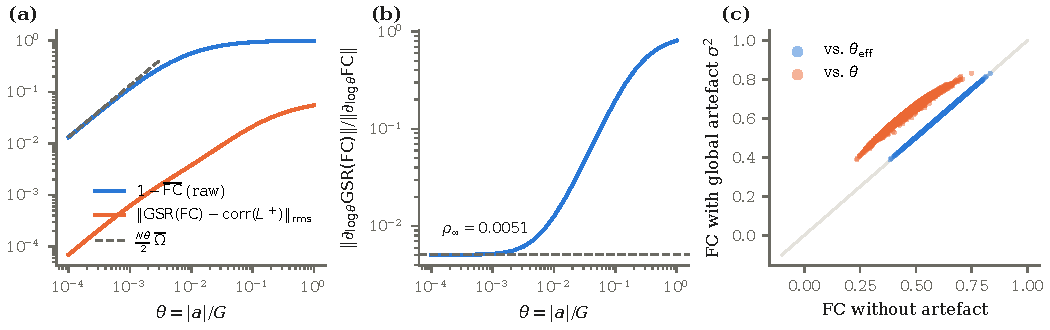
\includegraphics[width=\textwidth]{figures/fig2_gsr.pdf}
  \caption{Proposition~\ref{prop:gsr} on the group structural connectome (Schaefer-100, $N=100$). (a) Raw FC approaches $\one\one^\top$ linearly in $\theta$ with slope $\tfrac N2\overline\Omega$ (dashed); after GSR, FC approaches the $\theta$-independent limit $\corr(L^+)$. (b) Ratio of the sensitivities to $\log\theta$ with and without GSR; it converges to $\rho_\infty=0.0051$ (dashed). (c) Off-diagonal FC entries with a global artefact of variance $\sigma^2=1/(N\theta)$ at $\theta=0.01$, against FC without the artefact at $\theta$ (orange) and at $\theta_{\mathrm{eff}}=\theta/(1+N\sigma^2\theta)$ (blue): the artefact is equivalent to a change of the distance to the bifurcation.}
  \label{fig:gsr}
\end{figure*}


%======================================================================
\section{Empirical consequences}\label{sec:empirical}

The propositions make four predictions that can be tested on data: (P1) FC dynamics and metastability, the observables commonly used to select $G$, do not require a nonlinear or critical system; (P2) improving the fit of FC does not make the physical distance $\delta$ identifiable; (P3) without GSR, an FC-based index of the dimensionless distance is a function of mean FC, and with GSR it becomes unreliable and model-dependent; (P4) additive coupling does not escape the confound. We then check the theory in the full nonlinear model (Sec.~\ref{sec:nonlinear}) and show what a temporal measurement of $\delta$ can recover (Sec.~\ref{sec:temporal}). The fitting procedures, parameter bounds and validation splits are given in Appendix~\ref{app:methods}; code is available at \url{https://github.com/YuririaCP/conectome}.

\subsection{Data}

\emph{Time series.} Resting-state BOLD signals of 7 subjects from the Human Connectome Project~\cite{VanEssen2013}, as distributed with \texttt{neurolib}~\cite{Cakan2023}: AAL2 parcellation with $N=94$ regions, repetition time $0.72\,$s, 1200 volumes per subject, band-pass filtered to 0.008--0.08\,Hz, with the matching structural connectome. Empirical mean FC is 0.373 and peak frequencies lie between 0.018 and 0.030\,Hz.

\emph{Connectomes.} Structural and functional connectomes of 200 HCP subjects released by Domhof and co-authors~\cite{DomhofData2021,Domhof2021}, Schaefer-100 parcellation~\cite{Schaefer2018}, four resting-state sessions per subject (two phase-encoding directions on two days), giving 800 FC matrices. These FC matrices were computed from ICA-FIX denoised, detrended and z-scored signals without band-pass filtering and without GSR, which matches the setting of Propositions~\ref{prop:rescale}--\ref{prop:gsr}. Group FC from two disjoint halves of the cohort correlates at $r=0.995$, and group FC from sessions 1--2 and 3--4 at $r=0.997$.

\subsection{FC dynamics are largely reproduced by a stationary linear process}\label{sec:fcd}

We computed functional connectivity dynamics (FCD)~\cite{Hansen2015} with windows of 60\,s and steps of 2\,s, and metastability as the standard deviation of the Kuramoto order parameter of the Hilbert phases~\cite{Shanahan2010}. We generated multivariate phase-randomized surrogates~\cite{Prichard1994}: the discrete Fourier transform of each subject's band-passed regional signals was multiplied, at each nonzero frequency below Nyquist, by a phase factor $e^{i\phi_f}$ with $\phi_f$ uniform on $[0,2\pi)$ and shared by all regions, and transformed back. This preserves exactly the sample auto- and cross-periodograms, hence the sample FC and all circular lagged covariances, and destroys any structure beyond them. The surrogates are thus realizations compatible with a stationary linear process with the same second-order statistics, which is the null hypothesis they test; we make no claim about the Gaussianity of individual finite realizations. Pooled over subjects, they reproduce the empirical FCD distribution (Kolmogorov--Smirnov distance 0.072; 0.097 after GSR) and the empirical metastability (0.175 against 0.176) [Fig.~\ref{fig:fcd}(a,b)].

Per subject, we compared each statistic with 39 surrogates (two-sided Monte Carlo tests, smallest attainable $p=0.025$). Metastability differed from its surrogate distribution at $p<0.05$ in 1 of 7 subjects, with no consistent sign (Fisher's combined $p=0.17$). The KS distance between the empirical and surrogate FCD exceeded the surrogate-to-surrogate null in 1 of 7 subjects (combined $p=0.18$). The spread of the FCD, a standard index of non-stationarity, was larger in the data than in the surrogates in all 7 subjects (sign test $p=0.016$), by 10\% on average, but significantly so in only 1 subject. FC dynamics and metastability, as used to select $G$, are therefore largely accounted for by a stationary linear process with the same second-order structure, with a small but consistent excess of FCD variability, in line with Ref.~\onlinecite{Liegeois2017} (P1). With 7 subjects this is a demonstration that these observables do not require criticality or nonlinearity, not an estimate of how much non-stationarity human resting-state data contain.

In the nonlinear Hopf model with homogeneous parameters, the FCD distance decreases monotonically with $G$, reaching 0.044 at $G=3.5$. At that coupling, however, mean FC is 0.815 against an empirical 0.373, and the correlation between model and empirical FC falls to 0.445. Selecting $G$ by FCD therefore selects a strong global level of correlation [Fig.~\ref{fig:fcd}(c)], as Proposition~\ref{prop:gsr}(a) predicts.

\begin{figure*}
  \centering
  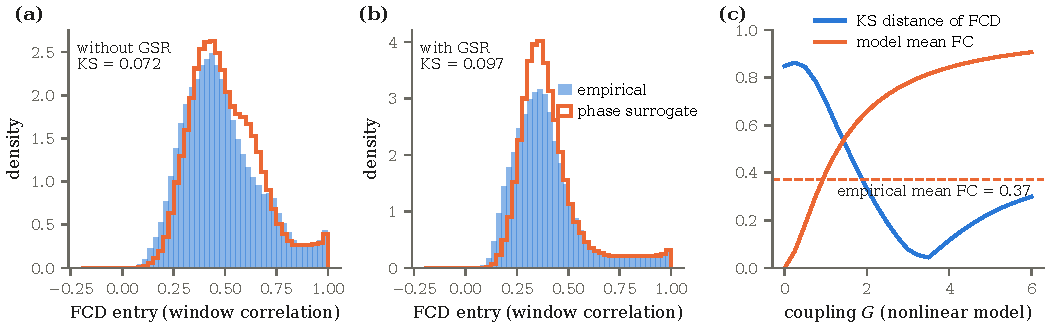
\includegraphics[width=\textwidth]{figures/fig3_fcd.pdf}
  \caption{FC dynamics are largely reproduced without a critical or nonlinear system (7 HCP subjects, AAL2). (a,b) Distribution of FCD entries (correlations between 60-s windows of FC), pooled over subjects, for the empirical data and for multivariate phase-randomized surrogates, which preserve the sample auto- and cross-periodograms and are compatible with a stationary linear process; KS is the Kolmogorov--Smirnov distance. (c) Nonlinear Stuart--Landau model with homogeneous parameters: the FCD distance is smallest at $G=3.5$, where model mean FC (0.815) is more than twice the empirical value (dashed).}
  \label{fig:fcd}
\end{figure*}

\subsection{Better fits, no identifiability}\label{sec:fit}

On the time-series data we fitted an effective connectivity (EC) with the update of Ref.~\onlinecite{Gilson2016}, using zero-lag and lagged covariances, region-wise $a_j$ and, in a second step, regional power spectra. On held-out subjects, model FC reached $r=0.764$ against a noise ceiling of 0.795, compared with 0.435 for the structural connectome. Two observations confirm (P2). First, the multivariate Ornstein--Uhlenbeck model ($\omega_j=0$) fitted as well as the Hopf model (held-out FC $r=0.766$ and 0.760 with EC alone; 0.771 and 0.729 when spectra were also fitted). Second, the fitted $a_j$ sat at the bounds of the admissible interval in 80 of 94 regions for the Hopf model and in 73 of 94 for the Ornstein--Uhlenbeck model, and the implied $\delta$ ranged from 0.03 to 0.15 between model variants of equal quality. The temporal information that a band-pass filter adds to FC (Proposition~\ref{prop:rescale}) is not enough to fix $\delta$.

On the 200-subject connectomes we fitted a symmetric diffusive EC to the group FC of half the cohort. On the other half, it reached $r=0.885$ with GSR (0.776 without), and individual FC was fitted with median $r=0.631$, against a test--retest ceiling of 0.894 and a group-template ceiling of 0.817. The fitted ratio was driven to $\theta\to0$: the median $\kappa$ across sessions was 0.0026, and with the SC-anchored diffusive model 84\% of sessions reached the lower bound.

\subsection{A relative criticality index is mean FC, or nothing}\label{sec:kappa}

For each of the 800 sessions we fitted a single dynamical parameter, $\theta$ (diffusive) or $\rho$ (additive), with the coupling matrix fixed at the group level, and computed $\kappa$. Without GSR, $\kappa$ was reliable across sessions (ICC(3,1) over four sessions 0.63; between days 0.65), but it was almost perfectly explained by mean FC: $r(\log\kappa,\overline{\FC})=-0.995$, and after partialling out mean FC the reliability fell to 0.30 [Fig.~\ref{fig:kappa}(a)]. This is Proposition~\ref{prop:gsr}(a) and (d): the index measures the global level of correlation (P3).

With GSR, the dependence on mean FC dropped ($r=-0.42$), as did the reliability (ICC over four sessions 0.47; between days 0.60). Replacing the group connectome by each subject's own connectome raised the four-session ICC to 0.65. Replacing it by the connectome of \emph{another} subject also raised it, to 0.60. The gain therefore reflects the stable individual structure that any connectome imprints on the fit, not the subject's dynamics [Fig.~\ref{fig:kappa}(b,c)]. Most importantly, $\kappa$ after GSR depended on the model: across subjects, the indices from additive coupling on the structural connectome and on the fitted EC correlated at $r=-0.36$, and those from additive and diffusive coupling on the same connectome at $r=0.57$ [Fig.~\ref{fig:additive}(b,c)]. A quantity that changes sign with modelling choices of equal fit quality is not a measurement of the brain.

\begin{figure*}
  \centering
  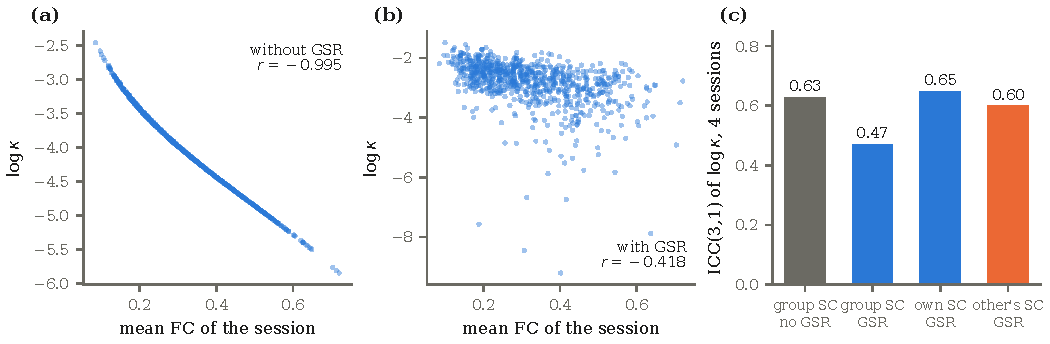
\includegraphics[width=\textwidth]{figures/fig4_kappa.pdf}
  \caption{The relative criticality index $\kappa$ over 800 sessions (200 HCP subjects, 4 sessions, Schaefer-100), fitted with the group connectome and one dynamical parameter per session. (a) Without GSR, $\log\kappa$ is a function of mean FC. (b) With GSR the dependence weakens. (c) Four-session reliability of $\log\kappa$: with GSR, using each subject's own connectome raises it, but so does the connectome of another subject (orange), so the gain is structural rather than dynamical.}
  \label{fig:kappa}
\end{figure*}

\subsection{Additive coupling does not escape}\label{sec:additive}

With additive coupling the critical mode is the Perron vector of the coupling matrix rather than $\one$, so one might hope to separate it from the global signal. Proposition~\ref{prop:perron} limits this hope, and the data remove it (P4). With the coupling anchored to the structural connectome, the transformation of the weights selected by the fit gave $\cos\angle(v,\one)=0.989$; for the untransformed group connectome the cosine is 0.82, and for the 200 individual connectomes it ranges from 0.46 to 0.91 [Fig.~\ref{fig:additive}(a)]. With a free symmetric EC, the diffusive model fitted held-out group FC better than the additive one ($r=0.885$ against 0.796 with GSR), and the partial correlations implied by the two fits agreed at $r=0.78$. In individual fits with GSR, 19\% of sessions placed the additive model at the bound $\rho\to1$.

\begin{figure*}
  \centering
  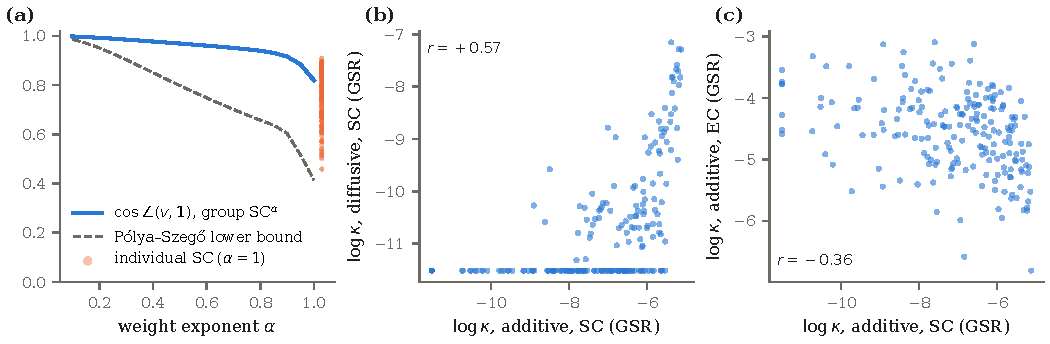
\includegraphics[width=\textwidth]{figures/fig5_additive.pdf}
  \caption{Additive coupling does not escape the confound. (a) Cosine between the Perron vector $v$ of the group connectome with weights raised to the power $\alpha$ and the uniform vector, with the Pólya--Szegő lower bound \eqref{eq:polya}; dots: the 200 individual connectomes with untransformed weights. (b,c) Subject-level $\log\kappa$ (mean over 4 sessions, with GSR) from three models of comparable fit: additive coupling on the structural connectome against diffusive coupling on the same connectome, where many sessions sit at the lower bound of $\kappa$ (b), and against additive coupling on the fitted EC (c).}
  \label{fig:additive}
\end{figure*}

\subsection{Beyond the linearization}\label{sec:nonlinear}

The propositions concern the linearized model with a common frequency. We tested the confound in the full model, Eq.~\eqref{eq:sl}, with heterogeneous frequencies, across the bifurcation. We used the AAL2 group connectome ($N=94$, normalized to mean strength 1), diffusive coupling with $G=0.2$, the empirical regional peak frequencies, $\beta=0.02$, and homogeneous $a$ from $-0.2$ to $0.05$. For each $a$ we ran 4 independent simulations of 50\,000\,s and computed zero-lag FC of $x=\operatorname{Re}z$ sampled at the TR. For each pair of neighbouring values of $a$ we measured the root-mean-square change of FC with and without GSR, after subtracting the sampling noise estimated from the spread across realizations (Fig.~\ref{fig:nonlinear}).

Below the bifurcation, nonlinear and linearized FC agree ($r\ge0.978$), and the ratio of the sensitivities with and without GSR follows the linear prediction (0.598 against 0.600, 0.413 against 0.409 and 0.258 against 0.255 on the three intervals furthest from the bifurcation). From $a=-0.03$ to $a=0.005$, raw FC changes by 3 to 14 times the sampling noise on each interval, while the change after GSR stays below it. The ratio reaches its minimum, 0.041, on the interval $[0,0.005]$ that contains the bifurcation. Heterogeneous frequencies, which lie outside the hypotheses of Proposition~\ref{prop:omega} and Theorem~\ref{thm:confound}, therefore do not undo the confound.

Above the bifurcation the picture changes. The evidence is in the absolute changes, not in the ratio alone [Fig.~\ref{fig:nonlinear}(b)]. On the three intervals from $a=0.005$ to $a=0.05$, FC after GSR changes by 0.017, 0.058 and 0.14 (root mean square, noise-corrected), that is, 2.4, 7.7 and 18 times its sampling noise. Raw FC changes by 0.24, 0.24 and 0.11 on the same intervals, and the last value is smaller because raw FC saturates (mean 0.91 at $a=0.05$). The ratios 0.069, 0.24 and 1.25 therefore combine a genuine increase of the sensitivity after GSR with a decrease of the raw sensitivity, and a ratio above one does not by itself mean that FC after GSR carries more information than raw FC. Band-passed FC gives the same pattern (ratios from 0.53 down to 0.058 up to the bifurcation, then 0.12, 0.42 and 2.1). What changes above the bifurcation is that FC acquires structure orthogonal to the global mode that depends on $a$; the next paragraph identifies a necessary condition for it. The global-mode confound is thus a property of the approach to the bifurcation from the damped side, which is where fitted operating points are usually read as distances to criticality. In the oscillatory regime FC after GSR depends on $a$, in line with the degeneracy reported there in terms of $K/\sqrt\lambda$ rather than of the distance itself~\cite{Alexandersen2025}.

\emph{Two regimes.} To determine what produces this dependence, we repeated the sweep for $G\in\{0.1,0.2,0.4\}$ and three frequency dispersions, $\omega_j=\bar\omega+s(\omega^{\rm emp}_j-\bar\omega)$ with $s\in\{0,0.5,1\}$, where $s=0$ is a common frequency (2 realizations of 20\,000\,s per point; Fig.~\ref{fig:regimes}). Below the bifurcation the change of FC after GSR stayed below its sampling noise in all nine conditions, while raw FC changed by up to 10 times its noise. Above the bifurcation the outcome depended on frequency heterogeneity. With a common frequency, FC after GSR stayed below the sampling noise up to $a=0.05$ for every $G$, although raw FC changed by up to 31 times its noise. With dispersion it became sensitive: on the interval $[0.02,0.05]$ its change was 2.4 to 4.7 times the noise for $s=0.5$ and 6.5 to 9.9 times for $s=1$, larger for weaker coupling. The global order parameter $R$ of the phases moves accordingly: at $G=0.2$ and $a=0.05$ the incoherence $1-R$ was 0.018, 0.023 and 0.038 for $s=0$, 0.5 and 1. A common frequency is the case covered by the theory: it drops out in a rotating frame (Proposition~\ref{prop:omega}), and for identical oscillators with diffusive coupling the synchronized state is uniform, so the dominant structure stays global even above the bifurcation. These observations support the interpretation that the non-global structure arises from incomplete synchronization of oscillators with different frequencies, that is, partial phase locking, but they do not resolve its spatial organization. The global-mode confound therefore holds on the damped side for any frequency profile, and on the oscillatory side only when frequencies are close to common.

\begin{figure*}
  \centering
  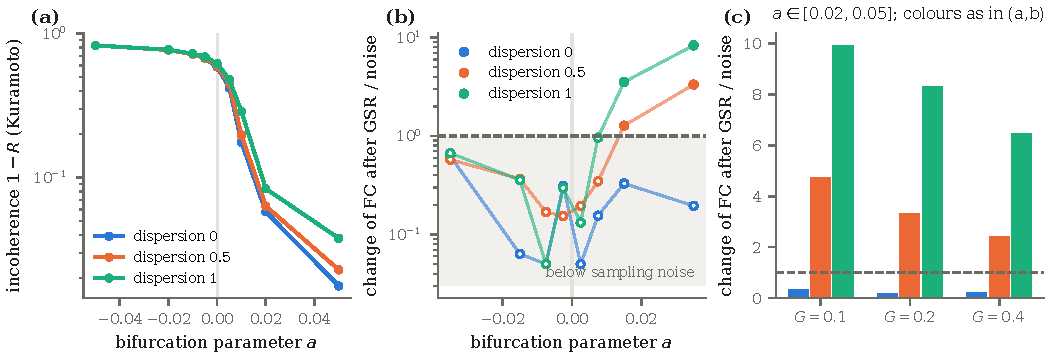
\includegraphics[width=\textwidth]{figures/fig6b_regimes.pdf}
  \caption{Two regimes of the confound (full nonlinear model, AAL2 group connectome, frequencies $\omega_j=\bar\omega+s(\omega^{\rm emp}_j-\bar\omega)$, 2 realizations of 20\,000\,s per point). (a) Incoherence $1-R$ of the Kuramoto order parameter at $G=0.2$ for three dispersions $s$. (b) Noise-corrected change of FC after GSR between neighbouring values of $a$, in units of its sampling noise, at $G=0.2$; open circles and shading: below the noise. (c) The same quantity on the interval $a\in[0.02,0.05]$ for three couplings $G$. With a common frequency ($s=0$) FC after GSR stays insensitive to $a$ on both sides of the bifurcation.}
  \label{fig:regimes}
\end{figure*}

\begin{figure*}
  \centering
  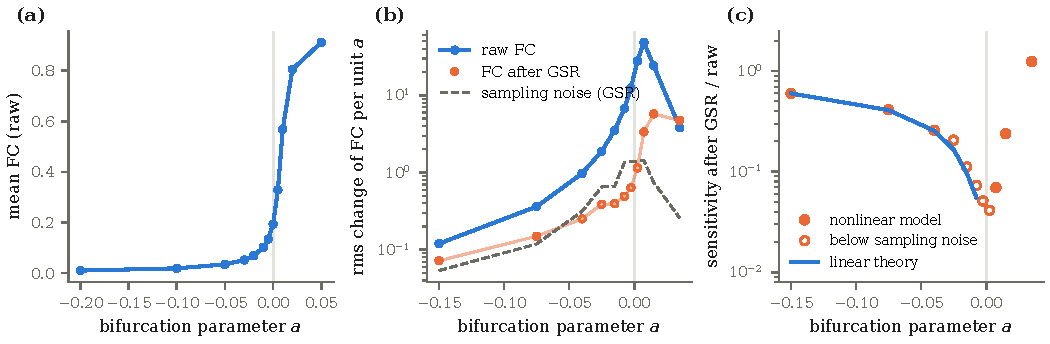
\includegraphics[width=\textwidth]{figures/fig6_nonlinear.pdf}
  \caption{The confound in the full nonlinear model with heterogeneous frequencies (AAL2 group connectome, $G=0.2$, homogeneous $a$; 4 realizations of 50\,000\,s per value). (a) Mean raw FC across the bifurcation at $a=0$. (b) Root-mean-square change of FC per unit $a$ between neighbouring values, without and with GSR, after subtracting sampling noise; open circles: changes below the sampling noise of FC after GSR (dashed). (c) Ratio of the two sensitivities, compared with the linear theory below the bifurcation.}
  \label{fig:nonlinear}
\end{figure*}

\subsection{Measuring $\delta$ in time}\label{sec:temporal}

The obstruction concerns zero-lag statistics, not the data. In the diffusive model with homogeneous damping, the global signal is the critical mode, so its autocorrelation decays at the physical rate $\delta$. We simulated the linearized model on the Schaefer-100 group connectome ($\theta=0.025$, common frequency 0.02\,Hz) along the family $(a,\omega,G,\beta)\mapsto c\,(a,\omega,G,\beta)$, $c\in\{0.5,1,2,4\}$. Along it the analytic FC is identical to machine precision, while $\delta=c|a|$ ranges from 0.01 to 0.08\,s$^{-1}$. From sessions of realistic length ($4\times1200$ volumes at $\mathrm{TR}=0.72$\,s, 5 realizations each), fitting $e^{-\delta\tau}\cos\omega\tau$ to the autocorrelation of the global signal over lags up to 60\,s recovered $\delta$ to within 8\% in every case [0.010, 0.020, 0.037 and 0.079\,s$^{-1}$; Fig.~\ref{fig:temporal}(a)]. The same fit applied to individual regions overestimated $\delta$ by an order of magnitude, because regional signals mix the critical mode with faster ones. After GSR it overestimated $\delta$ by a factor of about 27, because the critical mode has been removed.

This demonstration is favourable: neural signals are observed directly and nothing else is global. We therefore ran a recovery study under an fMRI-like observation model (Fig.~\ref{fig:recovery}; Appendix~\ref{app:recovery}). The ground truth was the linearized model with the empirical, heterogeneous frequencies, on three couplings: symmetric diffusive (Schaefer-100 group connectome, $l=r=\one$), directed diffusive (the effective connectivity of Sec.~\ref{sec:fit}, $r=\one$ but $l\neq\one$), and symmetric additive (group connectome, $l=r$ non-uniform), with $\delta\in\{0.01,0.03,0.1\}\,\mathrm s^{-1}$. The neural signals were convolved with a canonical hemodynamic response; a global physiological component (a slow arousal-like process plus a respiration-like band near 0.3\,Hz, with heterogeneous loading and the variance of the neural global signal) and white noise were added; and the data were high-pass filtered at 0.008\,Hz. A recording of the physiological component, correlated at 0.9 with the truth, was available. We estimated $\delta$ from the autocorrelation of a projection of the data with a fit whose model includes the hemodynamic response, the filter and white noise, over 10 realizations of $4\times1200$ volumes.

Three results stand out. First, without correction the global component inflates $\hat\delta$ when the critical mode is slow: median relative errors were $+1.0$, $+0.8$ and $+1.2$ at $\delta=0.01\,\mathrm s^{-1}$ for the three couplings. A fit that ignores the hemodynamics and the filter is worse still ($+1.9$ to $+2.4$). Second, regression on the recorded physiological signal removes most of the bias. With it, the median relative error lay between $-0.09$ and $+0.24$ for every coupling and every $\delta$, with interquartile ranges of about $\pm0.15$; with a single session of 1200 volumes the spread at least doubled. Third, GSR is the worst option: median errors of $+0.46$ to $+3.7$ for $\delta\le0.03\,\mathrm s^{-1}$, with wide spread, because the regression removes the mode whose rate is being estimated (Theorem~\ref{thm:confound}). Projecting on the critical vectors helped where they are not uniform: for additive coupling, without correction, the projection on $r=l$ reduced the error at $\delta=0.01\,\mathrm s^{-1}$ from $+1.21$ to $+0.61$, and for directed coupling the projection on $l$ reduced it at $\delta=0.03\,\mathrm s^{-1}$ from $+0.40$ to $+0.22$. After physiological regression the differences between projections were within the spread. We did not test the projection on $S^{-1}r$ of Proposition~\ref{prop:left}, which requires estimating the covariance. Under this observation model the physical distance is therefore recoverable to within roughly 20\%, but only when global physiology is regressed out with an independent recording rather than with the global signal itself.

\begin{figure*}
  \centering
  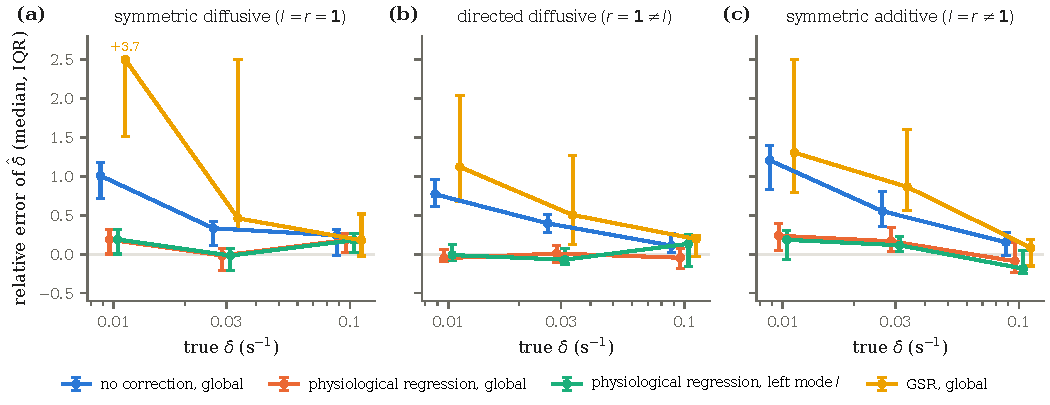
\includegraphics[width=\textwidth]{figures/fig8_recovery.pdf}
  \caption{Recovery of $\delta$ from synthetic fMRI-like data (canonical hemodynamic response, global physiological component, white noise, high-pass filter; $4\times1200$ volumes, 10 realizations). Median and interquartile range of the relative error of $\hat\delta$, from an observation-aware fit to the autocorrelation of the projected signal, for three couplings and four strategies: no correction with the global signal, regression on a recorded physiological signal with the global signal or with the left critical vector, and GSR. Values above 2.5 are clipped and labelled.}
  \label{fig:recovery}
\end{figure*}

For the empirical time series we report the same statistics only descriptively; they do not test the recovery of $\delta$. With only a high-pass filter at 0.008\,Hz, the global signal had a longer integrated autocorrelation time than the median region in all 7 subjects (2.6--4.2\,s against 2.0--2.8\,s), and GSR shortened the regional time scales in all 7 subjects (to 1.4--2.3\,s) [Fig.~\ref{fig:temporal}(b,c)]. In fMRI the global signal contains the hemodynamic response, respiration, cardiac pulsation, arousal and motion, any of which can lengthen its autocorrelation. Its longer time scale is therefore compatible with a slow critical mode but does not identify one, and these numbers should not be read as estimates of a neural relaxation rate. Separating a neural critical mode from these components, for example with concurrent physiological recordings and an explicit hemodynamic model, is the measurement problem that the global-mode confound poses; zero-lag FC cannot solve it.

\begin{figure*}
  \centering
  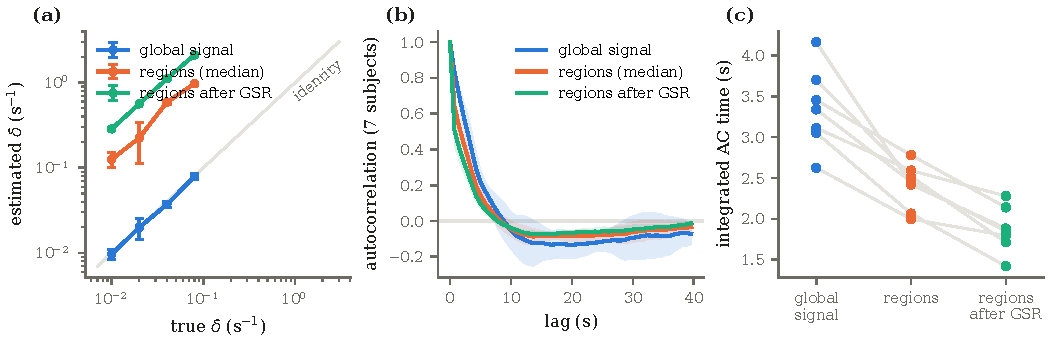
\includegraphics[width=\textwidth]{figures/fig7_temporal.pdf}
  \caption{Measuring the physical distance $\delta$ from temporal structure. (a) Linearized diffusive model on the group connectome along an FC-invariant family (Proposition~\ref{prop:rescale}): $\delta$ estimated from the autocorrelation of the global signal, of individual regions (median) and of regions after GSR, against the true $\delta$ (mean and s.d. over 5 simulated data sets of $4\times1200$ volumes). (b) Empirical autocorrelation of the global signal and of the regional signals (median over regions) before and after GSR; mean and s.d. over 7 subjects. (c) Integrated autocorrelation times per subject. Panels (b,c) are descriptive: the empirical global signal includes hemodynamic and physiological components, so its time scale is not an estimate of $\delta$.}
  \label{fig:temporal}
\end{figure*}

%======================================================================
\section{Discussion}\label{sec:discussion}

\emph{What FC can identify.} Zero-lag FC of a linear(ized) whole-brain model is the correlation matrix of a Gaussian graphical model~\cite{Lauritzen1996}. It identifies partial correlations and, given the coupling matrix, the dimensionless ratios $\theta_j=|a_j|/G$. It does not identify the time scale (Proposition~\ref{prop:rescale}), a common frequency (Proposition~\ref{prop:omega}), or the physical distance $\delta$ to the bifurcation. These statements are elementary, but they rule out reading a fitted $G$ or $a$ as a rate. They do not rule out the dimensionless distance $\theta$, or the index $\kappa$, which is a well-defined target under the model's assumptions.

\emph{What FC cannot separate.} The scale-free distance $\theta$ would still be a meaningful quantity, and with a fixed connectome it is identifiable in principle. The global-mode confound is what makes it hard to measure in practice. With excitatory coupling, the critical mode is positive and close to uniform (Propositions~\ref{prop:perron} and~\ref{prop:diffusive}); near the bifurcation $\theta$ enters FC only through its global level, which any global component with uniform loading can mimic (Proposition~\ref{prop:gsr}). Within the model this is a theorem. Its bearing on fMRI depends on an empirical premise: resting-state global fluctuations are associated with vigilance, respiration and motion~\cite{Liu2017}, and the confound applies to such components to the extent that their spatial loading is close to uniform (Remark~\ref{rem:loading}). Our analysis does not establish how close it is. What it does establish is that, near the bifurcation and to first order, any uniform component is exchangeable with a change of $\theta$, and that regressing out the global signal removes such a component together with the information about $\theta$. This offers a mechanism for the finding that model accuracy tracks the global signal~\cite{Aquino2022}, and for the degeneracy of the operating points fitted in different studies~\cite{Deco2017dynamics,Alexandersen2025}.

\emph{How to measure it.} Distance to criticality is a rate, and the natural observables are temporal (Sec.~\ref{sec:temporal}): the autocorrelation time of the slow mode, its growth as a control parameter is varied (critical slowing down~\cite{Scheffer2009}), or branching-type estimators~\cite{Wilting2018}. Our results add two requirements, and the recovery study (Sec.~\ref{sec:temporal}) quantifies them. First, the observable must be taken along the critical mode. Its variance lies along the right critical vector, close to the global signal, but its clock is the projection on the left critical vector (Proposition~\ref{prop:left}); the two coincide for symmetric coupling. Rabuffo and co-authors use the lag-one autocorrelation of the global signal~\cite{Rabuffo2025}, which is the right choice in the symmetric diffusive case. Second, global artefacts must be separated from the critical mode by means other than GSR. In our synthetic data, regression on a recorded physiological signal brought the error of $\hat\delta$ to within about 20\%, whereas GSR inflated it by up to a factor of five. Respiration, cardiac and arousal recordings, or data-driven removal of non-neural components, are the natural candidates; whether they suffice for real data is an empirical question that our simulations cannot settle. Information-geometric estimators~\cite{Du2026} face the same constraint when they weight regions by the leading eigenvector of the connectome, which by Proposition~\ref{prop:perron} is positive and, for the group connectome used here, has cosine 0.82 with the uniform vector.

\emph{Limitations.} The propositions concern the linearization and zero-lag statistics. Proposition~\ref{prop:rescale} holds for the nonlinear model, and simulations show that the confound survives nonlinearity and heterogeneous frequencies up to the bifurcation (Sec.~\ref{sec:nonlinear}). Above it, FC after GSR again depends on $a$ when frequencies are heterogeneous, consistent with partial phase locking; a theory of that regime is open. We did not include a hemodynamic model, and the empirical analyses use one parcellation per data set. The time-series analyses rest on 7 subjects and should be read as demonstrations of possibility, while the connectome analyses use 800 sessions. The Davis--Kahan bound~\eqref{eq:dk} can be loose for strongly heterogeneous damping, and we have no general estimate of $\rho_\infty(L)$, which on random graphs decreases with $N$. Finally, delays in the coupling~\cite{PonceAlvarez2024} break the commutation used in Proposition~\ref{prop:omega}, and their effect on the confound is open.

The critical-brain hypothesis is neither confirmed nor refuted by FC-based model fitting. It calls for a different observable.

\begin{acknowledgments}
Data were provided by the Human Connectome Project, WU-Minn Consortium (Principal Investigators: David Van Essen and Kamil Ugurbil; 1U54MH091657). Connectomes were obtained from EBRAINS (doi:10.25493/81EV-ZVT). This research received no specific funding.
\end{acknowledgments}

\section*{Data availability}
The connectomes are available from EBRAINS (doi:10.25493/81EV-ZVT); the HCP time series are distributed with \texttt{neurolib}. Analysis code, figures and the manuscript source are available at \url{https://github.com/YuririaCP/conectome}; processed results are regenerated by the scripts from the public data.


\appendix

\section{Fitting procedures}\label{app:methods}

All analyses use the diffusive model unless stated, noise amplitude $\beta=0.02$, and Fisher-$z$ averaging to form group FC. Scripts for every step are in the repository (\url{https://github.com/YuririaCP/conectome}).

\subsection{Time-series data (7 subjects)}

\emph{Targets.} Signals were band-passed to 0.008--0.08\,Hz with a second-order Butterworth filter applied forward and backward. FCD used windows of 60\,s and steps of 2\,s; metastability excluded 10 samples at each end to avoid edge effects of the Hilbert transform. Natural frequencies $\omega_j$ were set to the regional peak of the band-passed spectrum.

\emph{Model statistics.} Band-passed zero-lag and lagged covariances and regional spectra of the linearization were computed analytically, by integrating the cross-spectral matrix of the Ornstein--Uhlenbeck process against $|H(f)|^4$, where $H$ is the filter response (the square accounts for the forward-backward pass). Nonlinear simulations used Euler--Maruyama integration with step $\mathrm{TR}/8=0.09$\,s ($\mathrm{TR}/20$ in the comparison of linear and nonlinear FC), a 60\,s transient, and the same filter. Linear and nonlinear FC agreed at $r>0.98$ over the fitted range.

\emph{Homogeneous sweep.} $a\in\{-0.2,-0.1,-0.05,-0.02,-0.01,-0.005\}$ and $G\in[0,6]$ in steps of 0.1 with the analytic FC; nonlinear simulations at 25 values of $G$ in $[0,6]$ at the best $a$ (Fig.~\ref{fig:fcd}c).

\emph{Region-wise $a_j$.} L-BFGS-B on $(\log|a_j|,\log G)$ with bounds $|a_j|\in[10^{-4},1]$, $G\in[0.01,10]$, minimizing the mean squared error of FC plus that of the regional autocorrelations at lags of 3, 7, 14 and 28 TR (weight 1), plus $10^{-3}$ times the variance of $\log|a_j|$. Validation: fit on 4 subjects, test on the other 3.

\emph{Effective connectivity.} Starting from $G_0\,\mathrm{SC}$ with $G_0=3.3$ and homogeneous $a=-0.0696$ (the values of the previous step), all off-diagonal weights were updated by
$C\leftarrow\max\bigl(0,\,C+\varepsilon[(\mathrm{FC}^{0}_{\rm emp}-\mathrm{FC}^{0}_{\rm mod})+(\mathrm{FC}^{\tau}_{\rm emp}-\mathrm{FC}^{\tau}_{\rm mod})]\bigr)$,
with $\varepsilon=0.004$ and $\tau=2$\,TR, where $\mathrm{FC}^\tau$ is the normalized lagged covariance~\cite{Gilson2016}. The number of iterations (3000) was chosen by performance on the 3 held-out subjects; 88\% of the weights ended at zero. The noise ceiling is the correlation between the group FC of the two subject groups.

\emph{Joint fit of spectra.} Every 10 EC iterations, a damped Newton step per region adjusted $(\omega_j,\log|a_j|)$ to match the centroid and width of the empirical Welch spectrum (segments of 512 samples, normalized on 0--0.12\,Hz). Sensitivities were diagonal, estimated from two global perturbations; steps were clipped to 10\% in $\omega_j$ and 0.2 in $\log|a_j|$; parameters were bounded to $\omega_j/2\pi\in[0.005,0.12]$\,Hz and $|a_j|\in[10^{-3},1]$. ``At the bounds'' in Sec.~\ref{sec:fit} refers to these intervals. The Ornstein--Uhlenbeck variant fixes $\omega_j=0$. The implied $\delta$ was 0.029 (Ornstein--Uhlenbeck, EC and spectra), 0.064--0.070 (region-wise $a_j$ and EC with homogeneous $a$), and 0.146 (Hopf, EC and spectra), in $\mathrm{s}^{-1}$.

\subsection{Connectome data (200 subjects, 800 sessions)}

\emph{Coupling matrices.} Structural connectomes were symmetrized, given zero diagonal, and normalized to mean node strength 1, so that $\theta$ is comparable across connectomes. The group connectome is the mean over all 200 subjects in the one-parameter fits of Sec.~\ref{sec:kappa}, and over subjects 1--100 when it serves as the starting point of the transformed connectomes and of the effective connectivity.

\emph{One-parameter fits.} For each session, $\theta$ (diffusive) or $\rho$ (additive) was fitted by bounded scalar minimization of the mean squared error over the upper triangle of FC, with $\log\theta\in[\log10^{-4},\log10^{3}]$ (or $[\log 10^{-5},\log10^3]$ in the refits with transformed connectomes) and $\rho\in[10^{-4},\,1-10^{-5}]$. GSR, when used, was applied identically to model and data FC by Eq.~\eqref{eq:gsr}. A session is ``at the bound'' when $\kappa<2\times10^{-4}$.

\emph{Transformed connectomes.} We searched $C=\mathrm{SC}^{\alpha}$ with $\alpha\in\{1,0.5,0.25\}$ or $C=\log(1+\mathrm{SC})$, and extra weights $\{1,2,4\}$ on interhemispheric and $\{1,3,10\}$ on homotopic links, selecting by the fit to the group FC of subjects 1--100.

\emph{Symmetric effective connectivity.} From the selected transformed connectome, $C\leftarrow\max(0,\,C+\varepsilon(\mathrm{FC}_{\rm emp}-\mathrm{FC}_{\rm mod}))$ followed by symmetrization, with $\varepsilon=0.02$ and 4000 iterations. The target was the group FC of sessions 1--2 of subjects 1--100, and evaluation used all sessions of subjects 101--200. For additive coupling, $C$ was rescaled after each step so that $\lambda_{\max}(C)\le0.999$.

\emph{Reliability.} ICC(3,1) of $\log\kappa$ over the four sessions, and between days after averaging the two sessions of each day. The control with another subject's connectome used a fixed random permutation of subjects.

\section{Recovery study}\label{app:recovery}

\emph{Ground truth.} Complex Ornstein--Uhlenbeck process $\mathrm dz=(A+i\,\diag\omega)z\,\mathrm dt+\mathrm dW$, discretized exactly at $\mathrm{TR}=0.72$\,s, with $A=G\,B-sI$, $G=0.5\,\mathrm s^{-1}$, and $B=-(\diag(C\one)-C)$ (diffusive) or $B=C/\lambda_{\max}(C)-I$ (additive), $C$ normalized to mean strength 1. Frequencies are the empirical regional peaks (AAL2), randomly reassigned for Schaefer-100. The shift $s$ was set by root finding so that $-\max\operatorname{Re}\operatorname{spec}$ of the full real Jacobian equals the target $\delta$.

\emph{Observation.} Convolution with the canonical double-gamma hemodynamic response (peaks at 6 and 16\,s, ratio 6); a physiological component $p=a/\mathrm{sd}(a)+0.7\,b/\mathrm{sd}(b)$, with $a$ an AR(1) process of time constant 20\,s and $b$ white noise band-passed to 0.25--0.35\,Hz, added with loadings $1+0.3\xi_j$ and scaled to the variance of the neural global signal; white noise with half the regional variance; second-order Butterworth high-pass at 0.008\,Hz applied forward and backward. The recorded regressor is $0.9\,p/\mathrm{sd}(p)+\sqrt{0.19}\,\xi$, filtered identically.

\emph{Estimation.} Projections on $\one/N$, on the right critical vector $r$ and on the left critical vector $l$ of $B$ (computed from the structural model, not from the full Jacobian with frequencies). Autocorrelation over lags up to 60\,s. The naive fit uses $e^{-\delta\tau}\cos\omega\tau$. The observation-aware fit uses the autocorrelation of a Lorentzian pair at $\pm\omega$ with width $\delta$, multiplied by the squared modulus of the hemodynamic response and the fourth power of the filter response, plus a white-noise fraction; $(\log\delta,\omega,$ white fraction$)$ were fitted by least squares from three starting values. Code: \texttt{src/recovery\_delta.py}.

\bibliography{refs}

\end{document}
